% !TEX root = ../proyect.tex

\chapter{Planificación}\label{cap:planificacion}

Este capítulo presenta la planificación del proyecto LinceUS Assistant. Se describe la Estructura de Descomposición del Trabajo (EDT), el diccionario EDT que define cada paquete de trabajo, el backlog del producto organizado por épicas y la planificación temporal en sprints.

% =====================================================
% SECCIÓN 1: ESTRUCTURA DE DESCOMPOSICIÓN DEL TRABAJO
% =====================================================

\section{Estructura de Descomposición del Trabajo (EDT)}\label{sec:edt}

La Estructura de Descomposición del Trabajo (EDT), o \textit{Work Breakdown Structure} (WBS), organiza jerárquicamente todo el trabajo necesario para completar el proyecto. El nivel 0 representa el proyecto completo, el nivel 1 los paquetes de trabajo principales y el nivel 2 las tareas individuales que componen cada paquete.

La Figura~\ref{fig:edt} muestra la EDT a nivel de paquetes de trabajo (nivel 0 y 1), compuesta por \textbf{8 paquetes}: 2 transversales (gestión e investigación) y 6 épicas de desarrollo. El desglose de cada paquete en tareas individuales (nivel 2) se detalla en el diccionario EDT de la Sección~\ref{sec:diccionario-edt}.

\begin{figure}[hbtp]
\centering
\resizebox{\textwidth}{!}{%
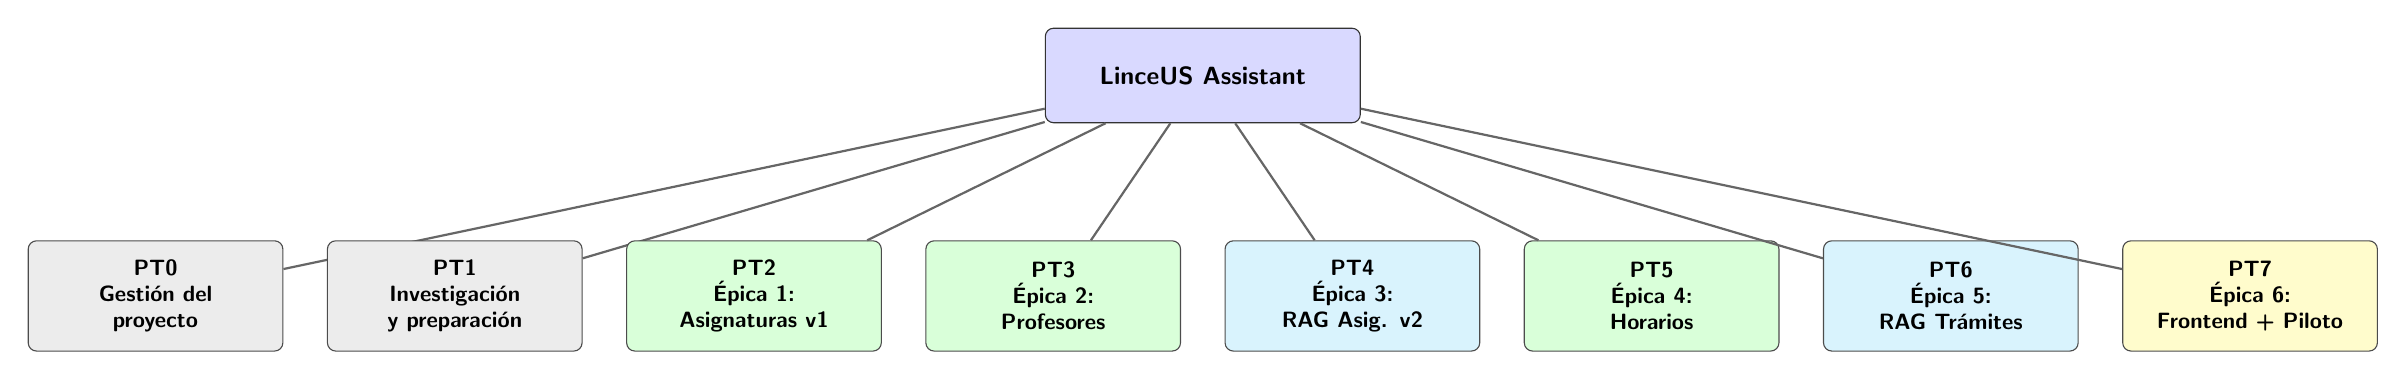
\begin{tikzpicture}[
    level 1/.style={sibling distance=38mm, level distance=28mm},
    every node/.style={font=\small\sffamily},
    root/.style={rectangle, draw=black!80, fill=blue!15, minimum width=40mm, minimum height=12mm, align=center, font=\small\sffamily\bfseries, rounded corners=3pt},
    pkg/.style={rectangle, draw=black!70, fill=#1, minimum width=32mm, minimum height=14mm, align=center, font=\footnotesize\sffamily\bfseries, rounded corners=3pt, text width=30mm},
    pkg/.default={orange!15},
    tasks/.style={font=\scriptsize\sffamily, text=black!60, align=center},
    edge from parent/.style={draw=black!60, thick}
]

\node[root] {LinceUS Assistant}
    child { node[pkg=gray!15] {PT0\\Gestión del\\proyecto} }
    child { node[pkg=gray!15] {PT1\\Investigación\\y preparación} }
    child { node[pkg=green!15] {PT2\\Épica 1:\\Asignaturas v1} }
    child { node[pkg=green!15] {PT3\\Épica 2:\\Profesores} }
    child { node[pkg=cyan!15] {PT4\\Épica 3:\\RAG Asig. v2} }
    child { node[pkg=green!15] {PT5\\Épica 4:\\Horarios} }
    child { node[pkg=cyan!15] {PT6\\Épica 5:\\RAG Trámites} }
    child { node[pkg=yellow!20] {PT7\\Épica 6:\\Frontend + Piloto} }
;

\end{tikzpicture}
}%
\caption{Estructura de Descomposición del Trabajo (EDT) — nivel de paquetes de trabajo.}
\label{fig:edt}
\end{figure}

% =====================================================
% SECCIÓN 2: DICCIONARIO EDT
% =====================================================

\section{Diccionario EDT}\label{sec:diccionario-edt}

El diccionario EDT define cada paquete de trabajo y sus tareas constituyentes, especificando su descripción, entregables y estimación de esfuerzo. Las estimaciones siguen la escala: \textbf{S} (Small, $\leq$1 semana), \textbf{M} (Medium, 1--2 semanas) y \textbf{L} (Large, 2--3 semanas).

% --- PT0 ---
\subsection{PT0 — Gestión del proyecto}\label{subsec:pt0}

Paquete transversal que abarca la planificación, seguimiento y documentación formal del proyecto a lo largo de todo su ciclo de vida.

\begin{table}[hbtp]
\centering
\small
\begin{tabular}{|l|l|p{7.5cm}|c|}
\hline
\textbf{ID} & \textbf{Tarea} & \textbf{Descripción y entregables} & \textbf{Est.} \\ \hline
0.1 & Planificación y seguimiento & Definición del alcance, elaboración de la EDT, planificación de sprints, seguimiento del progreso y gestión de riesgos. \textit{Entregable: anteproyecto, actas de seguimiento.} & L \\ \hline
0.2 & Redacción de la memoria & Redacción continua de la memoria del TFG: introducción, marco teórico, metodología, diseño, implementación, pruebas y conclusiones. \textit{Entregable: memoria del TFG.} & L \\ \hline
0.3 & Preparación de la defensa & Elaboración de las diapositivas de presentación, ensayo de la defensa y preparación de la demostración en vivo. \textit{Entregable: presentación, demo.} & M \\ \hline
\end{tabular}
\caption{Diccionario EDT — PT0: Gestión del proyecto.}
\label{tab:dict-pt0}
\end{table}

% --- PT1 ---
\subsection{PT1 — Investigación y preparación}\label{subsec:pt1}

Paquete que recoge el trabajo previo de investigación tecnológica, toma de decisiones y configuración del entorno de desarrollo.

\begin{table}[hbtp]
\centering
\small
\begin{tabular}{|l|l|p{7.5cm}|c|}
\hline
\textbf{ID} & \textbf{Tarea} & \textbf{Descripción y entregables} & \textbf{Est.} \\ \hline
1.1 & Estudio de tecnologías & Análisis comparativo de frameworks conversacionales (Rasa, Botpress, DeepPavlov), bases de datos (Supabase, PostgreSQL, motores vectoriales) y APIs de LLM (Gemini, OpenAI, DeepSeek). \textit{Entregable: tablas comparativas, decisión documentada.} & L \\ \hline
1.2 & Setup del entorno & Instalación y configuración de Python, Rasa, Supabase, Gemini API, Git/GitHub. Creación del repositorio y estructura inicial del proyecto. \textit{Entregable: entorno funcional, repositorio.} & M \\ \hline
1.3 & Diseño de la arquitectura & Definición de la arquitectura por capas, diseño de la base de datos, definición de interfaces entre componentes y protocolos de comunicación. \textit{Entregable: diagramas de arquitectura, esquema ER.} & M \\ \hline
\end{tabular}
\caption{Diccionario EDT — PT1: Investigación y preparación.}
\label{tab:dict-pt1}
\end{table}

% --- PT2 ---
\subsection{PT2 — Épica 1: Asignaturas v1 (BD estructurada)}\label{subsec:pt2}

Primera épica de desarrollo. Implementa la consulta de información básica de asignaturas (código, nombre, curso, créditos, tipología, duración) mediante consultas SQL sobre la base de datos estructurada, sin RAG.

\begin{table}[hbtp]
\centering
\small
\begin{tabular}{|l|l|p{7.5cm}|c|}
\hline
\textbf{ID} & \textbf{Tarea} & \textbf{Descripción y entregables} & \textbf{Est.} \\ \hline
2.1 & Esquema de datos en Supabase & Definir tablas de asignaturas (código, nombre, curso, créditos, tipología, duración) con restricciones de integridad y relaciones. \textit{Entregable: script SQL de creación.} & S \\ \hline
2.2 & Script de carga CSV + plantilla & Script Python/SQL con upsert, validaciones de obligatorios, tipos, duplicados y tildes. Plantilla vacía para nuevas titulaciones. \textit{Entregable: script de carga, plantilla CSV.} & M \\ \hline
2.3 & Ingesta del curso objetivo & Cargar $\sim$9 asignaturas del curso elegido (ETSII) y verificar integridad y relaciones. \textit{Entregable: datos cargados y validados.} & M \\ \hline
2.4 & Intents y entidades de consulta & Definir intents y entidades para ``calificación/evaluación/metodología/bibliografía de X'' con variaciones coloquiales y sinónimos. \textit{Entregable: ficheros NLU en YAML.} & M \\ \hline
2.5 & Acción Rasa (SQL) & Acción personalizada con consulta parametrizada a Supabase, normalización de nombres (fuzzy matching) y formateo de respuesta con fallback. \textit{Entregable: módulo actions.} & L \\ \hline
2.6 & Testing de la épica & Golden set $\geq$30 casos, unit tests y end-to-end. Objetivo: $\geq$90\% de acierto. \textit{Entregable: suite de tests, informe de resultados.} & M \\ \hline
2.7 & Documentación breve & Diagrama ER de datos y guía reproducible de carga (pasos y validaciones). \textit{Entregable: documentación técnica.} & S \\ \hline
2.8 & Preparación de RAG (inventario) & Lista de fuentes para proyectos docentes y criterios de inclusión/versión. \textit{Entregable: inventario de fuentes.} & L \\ \hline
\end{tabular}
\caption{Diccionario EDT — PT2: Épica 1 — Asignaturas v1.}
\label{tab:dict-pt2}
\end{table}

% --- PT3 ---
\subsection{PT3 — Épica 2: Profesores}\label{subsec:pt3}

Segunda épica. Permite consultar datos de contacto, despacho y horarios de tutorías del profesorado, con búsqueda por nombre o por asignatura.

\begin{table}[hbtp]
\centering
\small
\begin{tabular}{|l|l|p{7.5cm}|c|}
\hline
\textbf{ID} & \textbf{Tarea} & \textbf{Descripción y entregables} & \textbf{Est.} \\ \hline
3.1 & Esquema profesores/tutorías & Tablas \texttt{profesores} (nombre, departamento, correo, despacho) y \texttt{tutorias} (día, hora, modalidad) con FK hacia asignaturas. \textit{Entregable: script SQL.} & S \\ \hline
3.2 & Carga y normalización & Cargar CSV de profesores y tutorías; normalizar alias, tildes y abreviaturas; control de duplicados. \textit{Entregable: datos cargados.} & M \\ \hline
3.3 & Intents y entidades & Definir intents para ``Correo de\ldots'', ``Despacho de\ldots'', ``Tutorías de\ldots'' y ``¿Quién da [Asignatura]?''. \textit{Entregable: ficheros NLU.} & L \\ \hline
3.4 & Acciones SQL & Consultas por nombre y por asignatura; manejo de ambigüedades (varios profesores con nombre similar). \textit{Entregable: módulo actions.} & L \\ \hline
3.5 & Testing de la épica & Golden set $\geq$20 casos; $\geq$95\% de acierto; casos de alias y errores ortográficos menores. \textit{Entregable: suite de tests.} & M \\ \hline
\end{tabular}
\caption{Diccionario EDT — PT3: Épica 2 — Profesores.}
\label{tab:dict-pt3}
\end{table}

% --- PT4 ---
\subsection{PT4 — Épica 3: RAG Asignaturas v2}\label{subsec:pt4}

Tercera épica. Extiende la consulta de asignaturas con información extraída de los proyectos docentes (PDF) mediante técnicas de RAG: extracción, chunking, embeddings y búsqueda semántica.

\begin{table}[hbtp]
\centering
\small
\begin{tabular}{|l|l|p{7.5cm}|c|}
\hline
\textbf{ID} & \textbf{Tarea} & \textbf{Descripción y entregables} & \textbf{Est.} \\ \hline
4.1 & Inventario de fuentes & Mapa de proyectos docentes (URLs/PDF) y decisión de extracción (scraping vs curación manual). \textit{Entregable: inventario documentado.} & M \\ \hline
4.2 & Extracción y chunking & Parseo de PDF con pdfplumber, chunking semántico (800 caracteres, 100 de solapamiento) y metadatos (asignatura, año, sección, fecha de vigencia). \textit{Entregable: pipeline de extracción.} & M \\ \hline
4.3 & Embeddings en Supabase & Generación de embeddings con Gemini (\texttt{gemini-embedding-001}, 2000 dimensiones) y almacenamiento en pgvector con índices HNSW. \textit{Entregable: pipeline de vectorización.} & M \\ \hline
4.4 & Acción RAG con citas & Retrieval semántico + fallback por keywords; respuesta con cita (documento y sección) y umbral de confianza con fallback a enlaces útiles. \textit{Entregable: acción RAG integrada.} & L \\ \hline
4.5 & Testing de la épica & Anti-alucinación con golden set $\geq$40 casos, $\geq$90\% de precisión factual, pruebas de no-regresión al actualizar documentos. \textit{Entregable: suite de tests.} & M \\ \hline
\end{tabular}
\caption{Diccionario EDT — PT4: Épica 3 — RAG Asignaturas v2.}
\label{tab:dict-pt4}
\end{table}

% --- PT5 ---
\subsection{PT5 — Épica 4: Horarios}\label{subsec:pt5}

Cuarta épica. Permite consultar horarios de clases mediante una base de datos relacional con grupos, tramos horarios y aulas.

\begin{table}[hbtp]
\centering
\small
\begin{tabular}{|l|l|p{7.5cm}|c|}
\hline
\textbf{ID} & \textbf{Tarea} & \textbf{Descripción y entregables} & \textbf{Est.} \\ \hline
5.1 & Esquema horarios & Tablas \texttt{grupos\_clase}, \texttt{horarios} y \texttt{aulas} con claves foráneas y validación de solapes horarios. \textit{Entregable: script SQL.} & M \\ \hline
5.2 & Carga del curso & Cargar 1 curso ($\approx$4 grupos $\times$ 9 asignaturas) con validaciones de consistencia temporal. \textit{Entregable: datos cargados.} & S \\ \hline
5.3 & Intents y acciones & Consultas por asignatura, grupo y curso; formateo en tabla legible. \textit{Entregable: intents NLU y acciones Python.} & L \\ \hline
5.4 & Export CSV (opcional) & Exportar CSV del horario personal del alumno, si entra en alcance. \textit{Entregable: funcionalidad de exportación.} & L \\ \hline
5.5 & Testing de la épica & Golden set $\geq$30 casos; pruebas de rendimiento y de formato de salida. \textit{Entregable: suite de tests.} & M \\ \hline
\end{tabular}
\caption{Diccionario EDT — PT5: Épica 4 — Horarios.}
\label{tab:dict-pt5}
\end{table}

% --- PT6 ---
\subsection{PT6 — Épica 5: RAG Trámites}\label{subsec:pt6}

Quinta épica. Permite consultar información sobre trámites administrativos (matrícula, becas, certificados, convalidaciones) mediante RAG sobre páginas oficiales y documentos institucionales.

\begin{table}[hbtp]
\centering
\small
\begin{tabular}{|l|l|p{7.5cm}|c|}
\hline
\textbf{ID} & \textbf{Tarea} & \textbf{Descripción y entregables} & \textbf{Est.} \\ \hline
6.1 & Mapa de páginas & Identificar páginas oficiales y documentos relevantes; registrar fecha de vigencia de cada fuente. \textit{Entregable: mapa de fuentes.} & M \\ \hline
6.2 & Extracción/curación + chunking & Extraer contenido de webs y PDFs, normalizar, chunking con metacampos (tema, fecha, URL de origen). \textit{Entregable: pipeline de extracción.} & L \\ \hline
6.3 & Embeddings + acción RAG & Cargar embeddings; acción que siempre muestre fuente y fecha, y gestione discrepancias entre fuentes. \textit{Entregable: acción RAG de trámites.} & L \\ \hline
6.4 & Testing de la épica & Golden set $\geq$40 casos, pruebas de no-regresión y verificación de enlaces; $\geq$90\% de precisión factual. \textit{Entregable: suite de tests.} & M \\ \hline
\end{tabular}
\caption{Diccionario EDT — PT6: Épica 5 — RAG Trámites.}
\label{tab:dict-pt6}
\end{table}

% --- PT7 ---
\subsection{PT7 — Épica 6: Frontend + Piloto + Entrega}\label{subsec:pt7}

Sexta épica. Abarca el desarrollo de la interfaz web, la ejecución de un piloto con usuarios reales y la finalización de la documentación para la entrega.

\begin{table}[hbtp]
\centering
\small
\begin{tabular}{|l|l|p{7.5cm}|c|}
\hline
\textbf{ID} & \textbf{Tarea} & \textbf{Descripción y entregables} & \textbf{Est.} \\ \hline
7.1 & UI del widget web & Chat web conectado a Rasa mediante API REST; renderizado de respuestas enriquecidas (Markdown, tablas); accesibilidad básica (WCAG). \textit{Entregable: widget JS embebible.} & S \\ \hline
7.2 & Piloto y ajustes & Piloto con 5--10 estudiantes, recogida de feedback y ajustes de UX y flujos conversacionales; corrección de regresiones. \textit{Entregable: informe del piloto.} & M \\ \hline
7.3 & Memoria y defensa & Redacción final de la memoria (metodología, arquitectura, evaluación), elaboración de diapositivas y ensayo de defensa con métricas. \textit{Entregable: memoria final, presentación.} & L \\ \hline
\end{tabular}
\caption{Diccionario EDT — PT7: Épica 6 — Frontend + Piloto + Entrega.}
\label{tab:dict-pt7}
\end{table}

% =====================================================
% SECCIÓN 3: RESUMEN DE LA EDT
% =====================================================

\section{Resumen cuantitativo de la EDT}\label{sec:resumen-edt}

La Tabla~\ref{tab:resumen-edt} resume los paquetes de trabajo, el número de tareas y la distribución de esfuerzo estimada.

\begin{table}[hbtp]
\centering
\begin{tabular}{|l|l|c|c|c|c|}
\hline
\textbf{ID} & \textbf{Paquete de trabajo} & \textbf{Tareas} & \textbf{S} & \textbf{M} & \textbf{L} \\ \hline
PT0 & Gestión del proyecto & 3 & 0 & 1 & 2 \\ \hline
PT1 & Investigación y preparación & 3 & 0 & 2 & 1 \\ \hline
PT2 & Épica 1: Asignaturas v1 & 8 & 2 & 4 & 2 \\ \hline
PT3 & Épica 2: Profesores & 5 & 1 & 2 & 2 \\ \hline
PT4 & Épica 3: RAG Asignaturas v2 & 5 & 0 & 3 & 2 \\ \hline
PT5 & Épica 4: Horarios & 5 & 1 & 2 & 2 \\ \hline
PT6 & Épica 5: RAG Trámites & 4 & 0 & 2 & 2 \\ \hline
PT7 & Épica 6: Frontend + Piloto & 3 & 1 & 1 & 1 \\ \hline
\hline
\multicolumn{2}{|l|}{\textbf{Total}} & \textbf{36} & \textbf{5} & \textbf{17} & \textbf{14} \\ \hline
\end{tabular}
\caption{Resumen cuantitativo de la EDT por paquete de trabajo.}
\label{tab:resumen-edt}
\end{table}

% =====================================================
% SECCIÓN 4: BACKLOG
% =====================================================

\section{Backlog del producto}\label{sec:backlog}

El backlog del producto se deriva directamente de la EDT y organiza las épicas de desarrollo por prioridad. Cada épica se implementa de forma secuencial, de modo que las funcionalidades se entregan de forma incremental siguiendo el marco SCRUM adaptado descrito en el Capítulo~\ref{cap:metodologia}.

La priorización responde a dos criterios:

\begin{enumerate}
    \item \textbf{Valor para el usuario}: Las épicas que cubren las consultas más frecuentes de los estudiantes (asignaturas, profesorado) se implementan primero.
    \item \textbf{Dependencia técnica}: Las épicas que requieren infraestructura previa (como RAG, que depende de la base de datos vectorial) se planifican después de que dicha infraestructura esté operativa.
\end{enumerate}

La Tabla~\ref{tab:backlog-prioridad} muestra el orden de prioridad de las épicas.

\begin{table}[hbtp]
\centering
\begin{tabular}{|c|l|l|c|}
\hline
\textbf{Prioridad} & \textbf{Épica} & \textbf{Dependencia} & \textbf{Sprints est.} \\ \hline
1 & Asignaturas v1 (BD estructurada) & --- & S1--S8 \\ \hline
2 & Profesores (contacto, tutorías) & Épica 1 (esquema BD) & S9--S12 \\ \hline
3 & RAG Asignaturas v2 (proyectos docentes) & Épica 1 (inventario fuentes) & S12--S14 \\ \hline
4 & Horarios (BD relacional) & Épica 2 (profesores) & S15--S16 \\ \hline
5 & RAG Trámites & Épica 3 (pipeline RAG) & S17--S19 \\ \hline
6 & Frontend + Piloto + Entrega & Todas las anteriores & S19--S21 \\ \hline
\end{tabular}
\caption{Priorización del backlog por épicas.}
\label{tab:backlog-prioridad}
\end{table}

% =====================================================
% SECCIÓN 5: PLANIFICACIÓN DE SPRINTS
% =====================================================

\section{Planificación de sprints}\label{sec:sprints}

El proyecto se organiza en sprints de \textbf{3--4 semanas de duración}, siguiendo una adaptación de SCRUM para un proyecto individual (véase Capítulo~\ref{cap:metodologia}). Cada sprint tiene un objetivo definido y produce un incremento funcional del sistema.

% TODO: Completar con los sprints reales ejecutados y sus resultados

% =====================================================
% SECCIÓN 6: CRONOGRAMA
% =====================================================

\section{Cronograma}\label{sec:cronograma}

% TODO: Añadir diagrama de Gantt o cronograma temporal con los hitos principales del proyecto
